\documentclass{article}

% preamble
\def\npart{IV}
\def\nyear{2019}
\def\nterm{Lent}
\def\draft{Unfinished course}
\def\nlecturer{Dr J.\ Wolf}
\def\ncourse{Connections between Model Theory and Combinatorics}

\usepackage{mathrsfs}
\usepackage{imakeidx}
\usepackage{marginnote}

\ifx \nauthor\undefined
  \def\nauthor{Bhavik Mehta}
\else
\fi

\author{Based on lectures by \nlecturer \\\small Notes taken by \nauthor}
\date{\nterm\ \nyear}
\title{Part \npart\ -- \ncourse}

\usepackage[utf8]{inputenc}
\usepackage{amsmath}
\usepackage{amsthm}
\usepackage{amssymb}
\usepackage{enumerate}
\usepackage{mathtools}
\usepackage{graphicx}
\usepackage[dvipsnames]{xcolor}
\usepackage{tikz}
\usepackage{wrapfig}
\usepackage{centernot}
\usepackage{float}
\usepackage{braket}
\usepackage[hypcap=true]{caption}
\usepackage{enumitem}
\usepackage[colorlinks=true, linkcolor=mblue]{hyperref}
\usepackage[nameinlink,noabbrev]{cleveref}
\usepackage{nameref}
\usepackage[margin=1.5in]{geometry}

% Theorems
\theoremstyle{definition}
\newtheorem*{aim}{Aim}
\newtheorem*{axiom}{Axiom}
\newtheorem*{claim}{Claim}
\newtheorem*{cor}{Corollary}
\newtheorem*{conjecture}{Conjecture}
\newtheorem*{defi}{Definition}
\newtheorem*{eg}{Example}
\newtheorem*{ex}{Exercise}
\newtheorem*{fact}{Fact}
\newtheorem*{law}{Law}
\newtheorem*{lemma}{Lemma}
\newtheorem*{notation}{Notation}
\newtheorem*{prop}{Proposition}
\newtheorem*{question}{Question}
\newtheorem*{rrule}{Rule}
\newtheorem*{thm}{Theorem}
\newtheorem*{assumption}{Assumption}

\newtheorem*{remark}{Remark}
\newtheorem*{warning}{Warning}
\newtheorem*{exercise}{Exercise}

% \newcommand{\nthmautorefname}{Theorem}

\newtheorem{nthm}{Theorem}[section]
\newtheorem{nlemma}[nthm]{Lemma}
\newtheorem{nprop}[nthm]{Proposition}
\newtheorem{ncor}[nthm]{Corollary}
\newtheorem{ndef}[nthm]{Definition}

% Special sets
\newcommand{\C}{\mathbb{C}}
\newcommand{\N}{\mathbb{N}}
\newcommand{\Q}{\mathbb{Q}}
\newcommand{\R}{\mathbb{R}}
\newcommand{\Z}{\mathbb{Z}}

\newcommand{\abs}[1]{\left\lvert #1\right\rvert}
\newcommand{\norm}[1]{\left\lVert #1\right\rVert}
\renewcommand{\vec}[1]{\boldsymbol{\mathbf{#1}}}

\let\Im\relax
\let\Re\relax

\DeclareMathOperator{\Im}{Im}
\DeclareMathOperator{\Re}{Re}
\DeclareMathOperator{\id}{id}

\definecolor{mblue}{rgb}{0., 0.05, 0.6}

\swapnumbers
\reversemarginpar

\makeindex[intoc]

\let\oldmodels\models
\let\models\vDash
\let\nModels\nvDash

\newcommand{\named}[1]{\textbf{#1}\index{#1}}
\newcommand{\bonusnamed}[1]{\textbf{#1}\index{#1@*#1}}
\DeclareMathOperator{\tp}{tp}

\setcounter{section}{-1}
\tikzset{gaplabel/.style={fill=white, rectangle, inner sep=1mm}}

% and here we go!
\begin{document}
\maketitle

\tableofcontents

\clearpage
\section{Introduction}
% missing
Suppose we have a model $\mathscr{M} \models T$, then $\varphi(x,y)$ is said to have the $k$-OP if $\exists a_1, \dotsc, a_k, b_1, \dotsc, b_k$ such that $\models \varphi(a_i, b_j)$ iff $i \leq j$.
In the theory of abelian groups $\langle G, + , -, 0, A\rangle$ with the formula $\varphi(x,y) =$ `$x+y \in A$'.
Then $H \leq G$ are 2-stable, and $\bigcup_{i=1}^k (H + x_i)$ is $(k+1)$-stable.
\begin{ex}
  Show that if $A \subseteq G$ is $k$-stable, then so is $A+g$ for any $g \in G$. Moreover, $A^c$ is $(k+1)$-stable.
\end{ex}
\begin{lemma}
  Suppose $A_0, A_1 \subseteq G$ are $l$-stable and $k$-stable, respectively.
  Then $A_0 \cup A_1$ is $h(k,l)$-stable, where $h(k,l) = (k+l)2^{k+l}$.
\end{lemma}
\begin{proof}
  Suppose not. Then $\exists a_1, \dotsc, a_{h(k,l)}, b_1, \dotsc, b_{h(k,l)}$ such that $a_i + b_j \in A_0 \cup A$ iff $i \leq j$.
  \begin{center}
  \begin{tikzpicture}
    \node [label=left:$a_1$] at (0,0) {};
    \node [label=left:$a_2$] at (0,-1) {};
    \node [label=left:$a_3$] at (0,-2) {};
    \node [label=left:$a_4$] at (0,-3) {};
    \node [label=left:$a_{h(k,l)}$] at (0,-5) {};

    \node [label=right:$a_1$] at (2,0) {};
    \node [label=right:$a_2$] at (2,-1) {};
    \node [label=right:$a_3$] at (2,-2) {};
    \node [label=right:$a_4$] at (2,-3) {};
    \node [label=right:$a_{h(k,l)}$] at (2,-5) {};
  \end{tikzpicture}
  % complete bipartite
  \end{center}
  Since $a_i + b_j \in A_0 \cup A_1$ $\forall 1 \leq j \leq h(k,l)$ $\exists i_1 \in \{0,1\}$ and $D_1 = \{j : a_1 + b_j \in A_{i_1}\}$ with $|D_1| \leq h(k,l)/2$. Label $D_1$ as $j_1 < j_2 < \dotsb < j_{D_1}$ and define new sequences
  \begin{align*}
    a_1', \dotsc, a_{|D_1|}' &= a_1, a_{j_2}, \dotsc, a_{j_{|D_1|}} \\
    b_1', \dotsc, b_{|D_1|}' &= b_{j_1}, b_{j_2}, \dotsc, b_{j_{|D_1|}}. \\
  \end{align*}
  By pigeonhole, $\exists i_2 \in \{0,1\}$ and $D_2 = \{j | a_2' + b_j' \in A_{i_2}\}$.
  Label $D_2$ as $s_1 < s_2 < \dotsb < s_{|D_2|}$ and define new sequences
  \begin{align*}
    a_1^2 , \dotsc, a_{|D_2|}^2 &= a_1', a_2', a_{S_3}', \dotsc, a_{S_{|D_2|}}' \\
    b_1^2 , \dotsc, b_{|D_2|}^2 &= b_{S_1}', b_{S_2}', b_{S_3}', \dotsc, b_{S_{|D_2|}}' \\
  \end{align*}
  After $k+1$ steps, we will have sequences
  \begin{align*}
    a_1^{k+l}, \dotsc, a_t^{k+l}
    b_1^{k+l}, \dotsc, b_t^{k+l}
  \end{align*}
  with $t \geq \frac{h(k,l)}{2^{k+l}} = k+l$ such that $\forall 1 \leq j < s \leq t$, $a_s^{k+1} + b_j^{k+l} \notin A_0 \cup A_1$ and $\forall 1 \leq s \leq j \leq t$, $a_s^{k+l} + b_j^{k+l} \in A_{i_s}$.

  By pigeonhole again, either $\abs{\{s \mid i_s = 0\}} \geq l$ or $\abs{\{s \mid i_s = 1\}} \geq k$ contradicting the fact that $A_0$ ($A_1$) was $l$ ($k$)-stable.
\end{proof}
The typical model theoretic way of working with this is
\begin{defi}
  A formula $\varphi(x,y)$ is said to have the order property (OP) if there are sequences $(a_i)_{i < \omega}$, $(b_j)_{i < \omega}$ such that $\models \varphi(a_i,b_j)$ iff $i < j$.
\end{defi}
\begin{ex}
  Show that any Boolean combination of stable formulas is stable.
\end{ex}
\begin{defi}
  A theory has the OP if some formula in some model of the theory has the OP.
  A theory is stable if it does not have the OP.
\end{defi}
% 1.3
\subsection{Characterisation in terms of trees}
A tree in the set theoretic sense is simply a partial order $(P, \lhd)$ such that $\forall p \in P$, $\set{q \in P: q \lhd p}$ is a well-order.
\begin{notation}
  \begin{align*}
    2^{< n} &= \bigcup_{i < n} \{0,1\}^i \\
    \{0,1\}^0 = \langle \rangle \text{ the empty string}\\
    2^i = \{0,1\}^i
  \end{align*}
  % draw tree: n = 3, no edges, binary shaped
  The set $2^{< n}$ has a natural tree structure: $\rho \unlhd \eta$ iff $(\rho = \langle \rangle)$ or $\rho$ is an initial segment of $\eta$.
  If $\eta = \langle \eta_1, \dotsc, \eta_i \rangle$ , $j \in \{0,1\}$ then $\eta \wedge j = \langle n_1, \dotsc, n_i, j\rangle$.
\end{notation}
\begin{defi}
  Given a graph $\Gamma = \langle V, E \rangle$, the tree bound $d(\Gamma)$ is the least integer $d$ such that there do not exist sequences $(a_\eta)_{\eta \in 2^d}, (b_\rho)_{\rho \in 2^{<d}}$ of elements of $V$ with the property that for each $\eta \in 2^d, \rho \in 2^{< d}$, if $\rho \lhd \eta$, then $a_\eta b_\rho \in E$ iff $\rho \wedge 1 \unlhd \eta$.
\end{defi}
\begin{eg}
  A graph has tree bound $2$ if it does not contain the following:
  % see pic
\end{eg}
\begin{thm}[Shelah 1978, Hodges 1996, Alon et al 2018]
  For each $k$, $\exists d = d(k)$ such that if $\Gamma$ is a $k$-stable graph, then $d(\Gamma) \leq d$.
  (We will get $d(k) = 2^k + 1$, Hodges gives $2^{k+2} - 2$).
\end{thm}
Conversely, if $\Gamma$ contains the $2^k$-OP, then it contains a tree of height $k$.
$k=2$, % picture

More generally, a formula $\varphi$ admits a tree of height $d$ if $\exists (a_\eta)_{\eta \in 2^d}, (b_\rho)_{\rho \in 2^{< d}} \in M$ such that if $\rho \lhd \eta$, then $\models \varphi(a_\eta, b_\rho) \leftrightarrow \rho \land 1 \unlhd \eta$.

If $G$ has the $2^k$-OP, then it admits a tree of height $k$.

Want to show: If $G$ admits a tree of height $2^k + 1$, then $G$ has the $k$-OP.
% in the k=2 case, b<>, b1 is one class and a10, a11 is the other
Unfortuately, the $k=2$ case doesn't immediately generalise.
\begin{exercise}[Ramsey lemma]
  Suppose $p,q$ are positive integers and $T$ is a tree of height $p+q-1$ whose internal nodes are coloured red and blue.
  Then there is a subtree of height $p$ all of whose internal nodes are red or a subtree of height $q$ all of whose internal nodes are blue.
\end{exercise}
\begin{proof}
  Induction on $k$, where the induction statement is that the result is true, with one class a subset of leaves and the other class a subset of internal nodes.
  Assume $I(k)$, and we want $I(k+1)$.
  Given a leaf $y$, colour an internal node red if it is connected to $y$ by an edge in $G$, and blue otherwise.
  Use the Ramsey lemma on our tree, which has height $2(2^k + 1) - 1$, giving two cases
  \begin{itemize}
    \item Case 1: there is a leaf $y$ such that we get a red subtree $T'$ of height $2^k + 1$, say its root is $x$ (include the leaves too).
      Let $T''$ be the subtree of $T'$ rooted at the left child of $x$.
      Note that $T''$ has height $2^k$

      Let $X', Y'$ be the set of leaves, nodes of $T''$, respectively
      Note that no element of $Y'$ connects to $\eta$ in $G$.
      By the inductive hypothesis, we find $X_0 \subseteq X'$, $Y_0 \subseteq Y'$ that give a half graph of height $k$.

      Observe $y \in Y_0$. Let $X = X_0 \cup \{x\}$, $Y = Y_0 \cup \{y\}$.
      $y$ is connected to everything in $X_0$ but $x$ is connected to nothing in $Y_0$, giving the required halfgraph.
    \item Case 2: Suppose no leaf $y$ produces a red subtree of height $2^k + 1$.
      Say $x$ is the root of $T$, and say $T'$ is the subtree rooted at the right child of $x$, and consider only the leaves of $T'$.

      Pick a leaf of $T'$. This, by assumption, induces a blue subtree $T''$ in $T'$ of height $2^k$ in $T'$.

      By the inductive hypothesis, there are $X_0,Y_0$ which give a halfgraph of height $k$ using $X = \{x\} \cup X_0$, $Y = \{y\} \cup Y_0$ (attached to the front). \qedhere
  \end{itemize}
\end{proof}
\begin{exercise}
  Show that the theory of the random graph is unstable.
\end{exercise}
\subsection{Characterisation of stability in terms of types}
\begin{defi}
  Let $\mathscr{M} \models T$, $A \subseteq M$ a set of parameters, $\varphi(x,y)$ a formula.
  Then a (partial) $\varphi$-type over $A$ is a collection of formulas of the form $\varphi(x,a)$, $\neg \varphi(x,a)$ for some $a \in A$.
\end{defi}
\begin{defi}
  A complete $\varphi$-type over $A$ is a maximal consistent partial type over $A$ (i.e.\ $\forall a \in A$, either $\varphi(x,a)$ or $\neg \varphi(x,a)$ is in the type).
  Let $S \varphi(A)$ denote the space of complete $\varphi$-types over $A$.
\end{defi}
\begin{eg}
  $G = \langle V,E \rangle$, $A \subseteq V$, $\varphi(x,y) = E(x,y)$. Suppose $A = \{a_1,a_2,a_3,a_4\}$
  Then a possible type is $p(x) = \{E(x,a_1), E(x,a_2), \neg E(x,a_3)\}$, and the type defines the set of vertices which connect to $a_1$ and $a_2$ but not to $a_3$.
  \begin{center}
    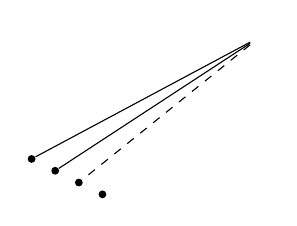
\begin{tikzpicture}
      \begin{scope}[every node/.style={inner sep=1pt, fill=black, circle}, xscale=0.3, yscale=0.15]
        \node (a4) at (0,0) {};
        \node (a3) at (-1,1) {};
        \node (a2) at (-2,2) {};
        \node (a1) at (-3,3) {};
      \end{scope}
      \node (x) at (2,2) {};
      \draw (x) -- (a1);
      \draw (x) -- (a2);
      \draw [dashed] (x) -- (a3);
    \end{tikzpicture}
  \end{center}
  $p(x)$ is not complete, but if, say, $\neg E(x,a_4)$ were added, then it is a complete $E$-type over $A$.
\end{eg}
% lecture 4
\begin{defi}
  Let $b \in M$, $A \subseteq M$. Then the type of $b$ over $A$ is the collecitno of all formulas with parameters in $A$ that are satisfied by $b$:
  \begin{equation*}
    \tp_\varphi(b/A) \coloneqq \{\varphi(x,a) \mid a \in A, \models \varphi(b,a)\}.
  \end{equation*}
\end{defi}
We have
\begin{equation*}
  S\varphi(A) \supseteq \{\tp_\varphi(b/A) \mid b \in M\}.
\end{equation*}
\begin{ex}\leavevmode
  \begin{enumerate}[label=(\roman*)]
    \item Prove the Erd\H{o}s-Makkai theorem:
      Let $A$ be an infinite set and let $\mathcal{F} \subseteq \mathcal{P}(A)$ such that $|\mathcal{F}| > |A|$. Then there are sequences $(a_i)_{i < \omega}$, $a_i \in A$, $(F_j)_{j < \omega}$, $F_j \in \mathcal{F}$ such that either
      \begin{align*}
        \text{either }a_i \in F_j &\leftrightarrow j < i \; \forall i,j \in \omega
        \text{or }a_i \in F_j &\leftrightarrow i < j \; \forall i,j \in \omega
      \end{align*}
    \item Deduce that if $|S\varphi(A)| > |A|$, then $\varphi(x,y)$ is unstable.
  \end{enumerate}
\end{ex}
\begin{thm}
  Let $G = (V,E)$ be an infinite graph. Suppose $\exists$ countable $A \subseteq V$ such that
  \begin{equation*}
    \abs{\{\{a \in A \mid E(a,b)\} \mid b \in V\}} > \aleph_0.
  \end{equation*}
  Then $G$ contains an infinite halfgraph.
\end{thm}
\begin{proof}
  Pick an uncountable sequence $(c_i)_{i < \omega_1}$, of distinct elements of $V$, each inducing a different partition of $A$.
  By induction on $n < \omega$, we define an increasing sequence of countable sets $A_n \subseteq V$ as follows:
  \begin{itemize}[label=--]
    \item $A_0 \coloneqq A$
    \item having constructed $A_n$ for some $n \geq 0$, we choose $A_{n+1} \supseteq A_n$ such that $\forall$ finite $B \subseteq A_n$, every partition of $B$ which is induced by a vertex in $V$ is already induced by a vertex in $A_{n+1}$.
  \end{itemize}
  Remark: $A_{n+1}$ is countable, since there are countably many $B$, and we only need to add in one vertex each.
  \begin{center}
    \begin{tikzpicture}[scale=1.8]
      \draw (0,0) ellipse (3.5cm and 2.5cm);
      \draw (-0.5,0.4) ellipse (2.5cm and 1.7cm);
      \draw (-0.9,0.7) ellipse (1.2cm and 0.7cm);
      \draw (0.3,0.2) circle (0.8);
      \node [gaplabel] at (-0.9,1.4) {$A_0=A$};
      \node [gaplabel] at (-0.5,-1.3) {$A_n$};
      \node [gaplabel] at (0,-2.5) {$A_{n+1}$};
      \node [gaplabel] at (0.5,0.98) {$B$};
      \draw [bred, shift={(0.3,0.2)}] (130:0.8) -- (-50:0.8);
    \end{tikzpicture}
  \end{center}
  Claim: $\exists i < \omega_1$ such that $\forall n < \omega$, $\forall$ finite $B \subseteq A_n$, we can find two elements $v = v_{n,B}$ and $w = w_{n,B}$ in $A_{n+1} \setminus \{c_i\}$ such that $v$ and $w$ induce the same partition on $B$ but $E(c_i,v)$ and $\neg E(c_i,w)$.

  For now, assume this claim, and construct the halfgraph.
  Fix $c_* = c_i$ for $i < \omega$ in the claim. We will construct three vertex classes, and use a Ramsey argument to give the halfgraph. Construct sequences $(a_n)_{n < \omega}, (b_n)_{n < \omega}, (c_n)_{n < \omega}$ with $a_n, b_n, c_n \in A_{2n+2}$.
  Having completed step $n-1$, let
  \begin{equation*}
    B_n = \bigcup_{m < n} \{a_m, b_m, c_m\}.
  \end{equation*}
  Note that $B_n \subseteq A_{2(n-1)+2} = A_{2n}$.
  By choice of $c_*$, $\exists a_n, b_n \in A_{2n+1} \setminus \{c_*\}$ such that $E(c_*, a_n), \neg E(c_*, b_n)$ and $a_n$ and $b_n$ induce the same partition on $B_n$.

  To complete step $n$, choose $c_n \in A_{2n+2}$ such that it induces the same partition of $B_n \cup \{a_n, b_n\}$ as $c^*$. (Note $c^*$ and $c_n$ induce the same partition on $B_n$, but this doesn't have to be the same partition that $a_n$ and $b_n$ induce on $B_n$).

  Observe:
  \begin{itemize}
    \item if $m > n$, then $a_m$ and $b_m$ relate to $c_n$ in the same way: $E(a_m ,c_n) \leftrightarrow E(b_m, c_n).$ % yellow
    \item if $m \leq n$, $c_*$ and $c_n$ relate to $a_m$ and $b_m$ in the same way, and $\forall m$, $E(a_m, c^*)$ and $\neg E(b_m, c^*)$. % red
      So $E(a_m, c_n)$ and $\neg E(b_m, c_n)$ for all $m \leq n$.
  \end{itemize}

  If $ E(a_m, c_n)$ on an infinite subsequence, $E(b_m, c_n) \leftrightarrow n < m$. If not, $E(a_m, c_n) \leftrightarrow m \leq n$.

  Finally, it remains to prove the claim.
  Suppose the conclusion fails. Then $\forall i < \omega_1$, $\exists n < \omega$, $\exists$ finite $B \subseteq A_n$ such that whether or not $c_i$ connects to $v \in A_{n+1} \setminus \{c_i\}$ is entirely determined by the partition of $B$ induced by $v$.

  Replacing $(c_i)_{i<\omega_1}$ by a subsequence, may assume that $n$ is constant and $B$ is constant. Fix $n,B$.
  By construction, since $B$ is finite, $\exists$ finite $C \subseteq A_{n+1}$ such that every partition of $B$ is already induced by an element of $C$.
  \begin{enumerate}[label=(\arabic*)]
    \item By passing to a subsequence, may assume that all $(c_i)_{i < \omega_1}$ induce the same partition on $C$.
    \item Any two $c_i$s induce distinct partitions on $A$, so $\exists a_* \in A$ such that $E(c_i, a_*)$ but $\neg E(c_j, a_*)$.
    \item By choice of $C$, there is $a_{**} \in C$ such that $a_*$ and $a_{**}$ induce the same partition on $B$.
    \item But $B$ is such that whether or not $v \in A_{n+1} \setminus \{c_i\}$ is connected to $c_i$ is entirely determined by the partition it induces on $B$.
  \end{enumerate}

\end{proof}
\section{Applications of stability}
\subsection{Stable Ramsey/Erd\H{o}s-Hajnal}
\begin{defi}
  Let $A \subseteq 2^{<n}$ be closed under initial segments (CUIS) and let $G$ be a graph on $n$ vertices.
  We say $G$ \textbf{is a type tree}\index{type tree} on $A$ if there is an indexing $V = \{a_\eta : \eta \in A\}$ such that $\forall \eta \in A$, the following holds.
  \begin{enumerate}[label=(\arabic*)]
    \item If $\eta \wedge 0$ is in $A$, then $\neg E(a_\eta, a_{\eta \wedge 0})$
    \item If $\eta \wedge 1$ is in $A$, then $E(a_\eta, a_{\eta \wedge 1})$
    \item If $\sigma,\tau \in A$ and $\eta \lhd \sigma \lhd \tau$, then
      \begin{equation*}
        E(a_\eta, a_\sigma) \leftrightarrow E(a_\eta, a_\tau)
      \end{equation*}
  \end{enumerate}
  A type tree of $A$ has height $h$ if $A \subseteq 2^{<h}$ but $A \nsubseteq 2^{<h-1}$
\end{defi}
\begin{lemma}
  Every graph on $n$ vertices is a type tree on $A$ for some $A \subseteq 2^{<n}$ (CUIS).
\end{lemma}
\begin{proof}

  Let $a_{\langle \rangle}$ be an arbitrary element of $V$.
  Let $A_0 = \{a_{\langle\rangle}\}$, $X_{\langle\rangle} = V$.
  Set $X_1 = N_G(a_{\langle \rangle})$, $X_0 = V \setminus (N_G(a_{\langle\rangle}) \cup \{a_{\langle\rangle}\})$
  Observe $X_0$ and $X_1$ partition $V \setminus A_0$.

  Suppose we've constructed $A_0, A_1, \dotsc, A_m$ for $m \geq 0$, and that for each $\eta \in A_m$, we have a partition of $X_\eta$ with the following properties:
  \begin{enumerate}
    \item $\{X_{\eta \wedge i}: \eta \in A_m, i=0,1\}$ partition $V \setminus \bigcup_{i=0}^m \{a_\eta : \eta \in A_i\}$
    \item $\forall \eta \in A_m$, $X_{\eta \wedge 1} \subseteq N_G(a_\eta)$, $X_{\eta \wedge 0} \subseteq V \setminus (\{a_\eta\} \cup N_G(a_\eta)).$
  \end{enumerate}

  Now for each $\eta \in A_m$ and $i \in \{0,1\}$ let $a_{\eta \wedge i}$ be an arbitrary element of $X_{\eta \wedge i}$ be an arbitrary element of $X_{\eta \wedge i}$. If $X_{\eta \wedge i} \neq \emptyset$. Let $A_{m+1}$ be the set of all these elements.

  For each $\sigma \in A_{m+1}$, $i \in \{0,1\}$,
  \begin{align*}
    X_{\sigma \wedge 1} = N(a_0) \cap X_0 \\
    X_{\sigma \wedge 0} = (V \setminus (\{a_0\} \cup N_G(a_d))) \cap X_\sigma
  \end{align*}
  Check that the set $A = \bigcup_{i=1} A_i$ satisfies the properties of a type tree.
\end{proof}
\begin{defi}
  Say $G=(V,E)$ contains a type tree of height $h$ if $\exists V' \subseteq V$ such that the induced graph on $V'$ is a type tree of height $h$ on $A$ for some $A \subseteq 2^{<h}$ (CUIS).

  The tree height of $G$, denoted by $h(G)$ is the largest $h$ such that $G$ contains a type tree of height $h$.
\end{defi}
\begin{defi}
  Say $G = (V,E)$ contains a full binary type tree of height $t$ if $\exists V' \subseteq V$ such that the induced graph on $V'$ is a type tree on the set $2^{<t}$.
  The tree rank of $G$, $t(G)$ is the largest full binary type tree of height $t$.
\end{defi}
Observe that $d(G) \leq k$ then $t(G) \leq k$.

% \begin{thm}[Malliaris-Shelah, Malliaris-Terry]
%   For all integers $k$, $\exists c = c(k)$ and $\delta = \delta(k)$ such that the following holds. Let $n \geq 2$ be an integer and let $G$ be a $k$-stable graph on $n$ vertices. Then $G$ contains a clique or an independent set of size at least $c n^\delta$.
% \end{thm}
\printindex
\end{document}
